\chapter{Introduction}

\section{Stop Killing Games}
This report gathers and presents the evidence and argumentation for why governments should take action to preserve game ownership.
It includes a description of what killing a game involves,
examples of where games have been killed and counter-examples of games that have seen support ended in a responsible fashion,
a summary of the arguments made,
and a series of recommendations for how to protect game ownership.
We also include a glossary to explain technical or videogame specific terms.

\lm{Include a focused explanation of what this action is asking for, and what it is not asking for}
This document is an accompaniment to the Stop Killing Games campaign~\cite{stop-killing-games-2024},
which will target government action through petitions and contacting consumer rights groups.

\subsection{Videogames}
The first videogames were released in the latter half of the 20th century.
From videogames played in an amusement arcade, the industry changed, developing for home games consoles, PCs, and more recently handheld devices including mobile phones.
Globally, the videogames industry is worth £TODO\cn,
with an estimated TODO\cn players,
spending an average of TODO\cn on videogames and game related purchases annually.
Players encompass audiences from the very young to the very old, and gaming is popular across demographic groups\cn.
Videogames are a relatively new form of entertainment, but are becoming a central part of culture and art.
\lm{Is there debate on whether they are art or product?}

Early videogames were sold as physical products, such as cartridges that could be installed into a device, or on storage media such as CD-ROMs.
For games sold in this fashion, they could not be patched after sale any multiplayer capability was limited to local play.
It also meant that the task of keeping the game in a working state was left to the player who purchased it.
As long as they kept their console and media in good condition, they could keep playing the game as long as they wished.

More recently, internet connectivity has made it easier to connect games, and has enabled development of new features for singleplayer games such as online leaderboards.
Players could connect directly to each other's machines and engage in multiplayer games without needing to be in the same room.
As internet connections improved, it has become cheaper to sell and distribute videogames through online storefronts such as Steam, Google Play,
and more viable to include online connectivity features within games.
Even some physical games sold now only serve as an activation key for a game delivered over the internet\cn.

A major shift in the concept of videogames, brought about with improvements in internet connectivity is that it is easier for publishers to retain control of key game components.
As a result, games rely on the internet and on online components controlled by publishers, so the longevity of games is becoming tied to continued internet access.
These online components will not always be available:
there may be temporary service interruptions,
difficulties with international relations resulting in censorship of communications,
and at some point the publisher may choose to end support for these online components.
When an interruption occurs, players may lose access to part or all of a videogame,
this poses an unprecedented level of disruption for a consumer owned product.

Figure~\ref{fig:evolution} shows the change in technology over time.
From games that could exist entirely on one device, and be playable as long that device was in good condition,
to online games where players each could control the game in its entirety,
to modern online games where playability is dependent on continued support from the publisher.

\begin{figure}
    \caption{Evolution of games}%
    \label{fig:evolution}
    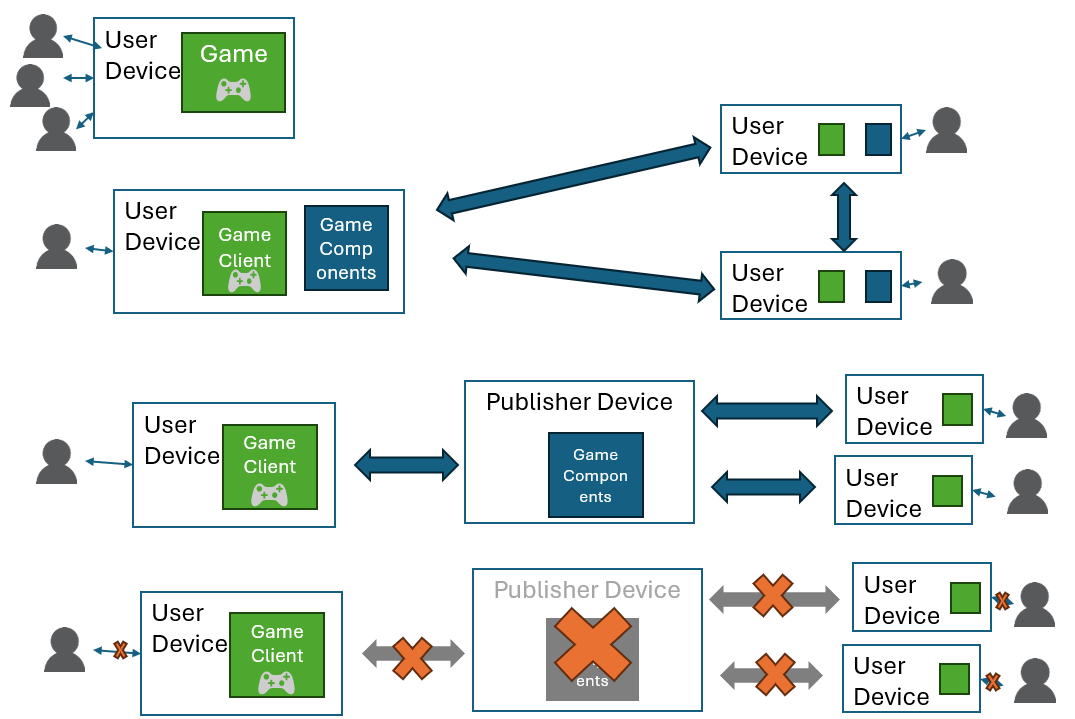
\includegraphics[width=1\textwidth]{images/evolution}
\end{figure}

\lm{This is a placeholder graphic.
It may be necessary throughout the report to use diagrams to illustrate the various ways that videogames are vulnerable, and how they can be protected.
Use a diagram early on to present the history of games, from running on one device, to the publisher having more control over the net.
Decide on a common visual language to represent various aspects and use these throughout}

During a game's servicing period
\lm{Is this the right term to use?}
minor disruptions will not cause a permanent loss of the product.
However, when a publisher ends support, this could permanently render a game unplayable.
We call this \emph{``Killing a Game''}.
Publishers argue that this is permitted under the license with which the game is sold.
Players argue that this is damaging a product that has been sold.
\lm{Make sure these two preceding sentences are correct and agreed upon terminology.}

The goal of this campaign is twofold:
\begin{enumerate}
    \item Settle the legal status of killing games ---
    Are publishers legally allowed to render a game completely unplayable when they choose to end support, and under what conditions is this legal or illegal.
    \item Guarantee playability of games sold after support ends ---
    Create a framework requiring publishers to take action when planning, developing and distributing games such that after the support period ends,
    players can keep playing their game in some form.
\end{enumerate}

We recognise that there will be cases where it may not be possible to ensure post-servicing playability of some game features.
What we are asking for is that the core parts of a game remain playable even after support ends.
In the remainder of this report we will provide examples of games that have been shut down appropriately, and games which have been killed outright.
We will also describe in more detail the action we would like to see applied to publishers.

% The goal of this campaign - how it will succeed
% ``If companies face penalties for destroying copies of games they have sold, this is very likely to start curbing this behavior.
% If a company is forced to allow customers to retain their games in even one country, implementing those fixes worldwide becomes a trivial issue for them.
% So, if destroying a game you paid for became illegal in France, companies that patched the game would likely apply the same patch to the games worldwide.
% An analogy to this process is how the ACCC in Australia forced Valve to offer refunds on Steam, so Valve ended up offering them to people worldwide as a result.
% ''
